% Le type de document: article, rapport...
\documentclass[a4paper]{report}

% Mettre les diffe'rents packages et fonctions que l'on utilise
\usepackage[utf8]{inputenc}
\usepackage[french]{babel}
\usepackage{amsmath}
\usepackage{amssymb}
\usepackage{graphics,color}
\usepackage{graphicx}
\usepackage{fancyhdr}
\pagestyle{fancy}
%bien inclure du code source
\usepackage{moreverb}
\usepackage{listings} % a inclure pour la fonction listing
\usepackage{textcomp} 
\usepackage{xcolor} % on en a besoin pour utiliser les couleurs
%avoir figure 1 et non figure1.1 et table 1 au lieu de table 1.1.1
\usepackage{url}
\newcommand{\lien}[1]{$\,$\footnote{$\,$\url{#1}}}
\usepackage{caption}
\captionsetup{figurewithin=none}  
\captionsetup{tablewithin=none}
% pour régler le header et footer
\fancyhead{}
\fancyfoot{}
\renewcommand{\chaptermark}[1]{\markboth{#1}{}}
\renewcommand{\sectionmark}[1]{\markright{#1}}

\lhead{\chaptername~\thechapter. \leftmark\\\textit{\rightmark}}

\chead{}
\rhead{

\includegraphics[height=1cm]{images/ecm.ps}
\includegraphics[height=1cm]{images/lif.ps}
} 
\lfoot{Ismaeil Abouljamal}
\cfoot{Rapport TFE 2011}
\rfoot{\thepage}
%helpers
\newcommand{\meet}{\wedge}
\newcommand{\join}{\vee}
\newcommand{\bottom}{\bot}
  % pouvoir mettre des formules mathématiques en gars 
\renewcommand{\textbf}[1]{\begingroup\bfseries\mathversion{bold}#1\endgroup}

%environnements
\newtheorem{definition}{Définition}[chapter]
\newtheorem{theorem}{Théorème}[chapter]
\newtheorem{proposition}{Proposition}[chapter]

\newenvironment{preuve}{\textbf{Démonstration}}{}

\begin{document}


%----------- A   C O M P L E T E R   P A R   L E S   A U T E U R S ------------


% Titre du rapport
\def\TitreRapport{
Tables 0/1 Associées Aux Treillis Démontables
}


% Pre'nom et nom de l'auteur
\def\NomsAuteurs{
Ismaeil Abouljamal
}

% Date du rapport (dans la même langue que le titre)
\def\DateRapport{
    10 juin 2011
}

% Nom des encadrants
\def\Encadrants{
    \textbf{Encadrant} \\
    François Brucker
}
% Nom du laboratoire
\def\Labo{
    LIF (UMR 6166)
}



% Résumeé en français avec mots-clés
\def\ResumeFrancais{
Dans ce rapport, on se place dans le cadre des treillis démontables et nous montrons une équivalence entre la notion de démontabilité sur cette structure et celle
de la table 0/1 associée.
Nous étendons par là la bijection existante entre les treillis démontables et leur systèmes de classes associés ; bijection qui a déjà été démontrée dans~\cite{par_clu} et~\cite{crow_free}.
Nous caractérisons les tables 0/1 correspondantes aux treillis démontables en montrant qu'une table 0/1 est démontable si et seulement s'il existe une permutation 
des lignes et/ou des colonnes n'admettant pas la configuration $\Gamma$. 
    \\[2mm]
    {\bf Mots-clés~: }classification, treillis démontables, système de classes, table 0/1, schéma d'élimination.
}


\thispagestyle{empty}
\begin{center}
\baselineskip=1.3\normalbaselineskip
{\bf\Large \TitreRapport}\\[8mm]
{\bf\large \NomsAuteurs}\\[1mm]
{\Labo}\\[4mm]
\begin{center}

\includegraphics[height=2cm]{images/ecm.ps}
\includegraphics[height=2cm]{images/lif.ps}
\end{center}
\Encadrants\\[10mm]

{\bf Résumé}
\end{center}
\ResumeFrancais\\[4mm]

%-------------------- Table de matières -------------------------
\tableofcontents

%-------------------- T E X T E   D U   R A P P O R T -------------------------

\chapter{LIF}

\section{Présentation}

Le Laboratoire d'Informatique Fondamentale de Marseille (LIF) est une unité mixte de recherche (UMR 6166) du CNRS, de l'université de Provence et de l'université de la Méditerranée. Au CNRS, le LIF est rattaché à l'Institut des sciences informatiques et de leurs interactions (INS2I) à titre principal et à l'Institut des Sciences Humaines et Sociales (INSHS), à titre secondaire. Le LIF comprend 78 membres permanents, et une trentaine de membres non permanents, répartis sur 2 sites principaux distants : le campus de Luminy et le technopôle de Château-Gombert. Le LIF est structuré en cinq équipes dont les thèmes couvrent une part significative de l'informatique contemporaine :

\begin{itemize}
 \item Bases de données et Apprentissage Automatique
 \item Combinatoire et Recherche Opérationnelle
 \item Modélisation et Vérification
 \item Systèmes complexes, automates et pavages
 \item Traitement Automatique du Langage Écrit et Parlé
 
\end{itemize}


Le master d'informatique de Marseille que j'ai suivi en parallèle avec ma troisième année à Centrale Marseille est adossé au LIF .

\section{Organigramme}
\begin{figure}
\begin{center}
\includegraphics[height=9cm]{images/orgalif.ps}
\end{center}
\caption{Organigramme du LIF}
\end{figure}

\chapter{Introduction}

\label{intro}

\begin{verse}
\og Le seul moyen de faire une méthode instructive et naturelle est de mettre ensemble les choses qui se ressemblent et de séparer celles qui diffèrent
les unes des autres\fg 

(Georges Louis Leclerc de Buffon. \textsc{Histoire Naturelle}~\cite{histoire}).
\end{verse}
Cette phrase montre l'enjeu de la classification~: rassembler les objets dans des classes bien séparées qui, une fois caractérisées, permettent 
une interprétation de données. Classiquement, les modèles utilisés pour relever ce défi sont les partitions et les hiérarchies de classes. Dans ces deux cas, les classes
 d'Objets -homogènes- sont automatiquement séparées car elles sont disjointes pour les partitions ; et/ou emboîtées dans le cas des hiérarchies.

Cependant, dans bien des cas pratiques, cette séparation stricte est préjudi\-cielle~: il arrive que l'on ait besoin qu'un objet appartienne à deux classes distinctes, sans qu'il soit
 seul dans sa classe, par exemple l'hybridation d'espèce. Une interprétation correcte doit absolument prendre en compte la relation existante entre l'hybride 
et ses parents (l'hybride ne peut ni \^etre interprété comme une nouvelle classe, ni appartenir seulement à la classe du père ou celle de la mère).

Des structures admettant le chevauchement  de classes existent. On citera par exemple~:
\begin{itemize}
 \item \textsc{Les pseudo-hiérarchies} (\cite{dur}) qui reposent sur la notion de \textsc{dissimilarité de Robinson} où les classes s'interprètent commme
 des intervalles d'un ensemble totalement ordonné ;
\item \textsc{Les hiérarchies faibles} (\cite{dia} et~\cite{band}) où l'intersection de trois classes est ramenée à l'intersection de deux d'entre-elles ;
\item \textsc{Systèmes de classes parcimonieux} (\cite{par_clu}) en bijection avec les treillis démon\-tables.
\end{itemize}


On se place dans le troisième cadre et nous avons étendu la bijection existante entre les treillis démontables 
et les systèmes de classes correspondants (\cite{crow_free} et~\cite{par_clu}) en démontrant la bijection entre les tables 0/1
 ordonnables et les systèmes de classes démontables.

La première partie (section~\ref{gene}) introduit les 3 structures (treillis - classes - tables) et quelques résultats généraux sur le sujet utiles pour la suite.
La deuxième partie (section \ref{structuredemonta}) introduit la notion de démontabilité et la bijection connue entre la structure treillis et la structure système de classe.
La troisième  partie quant à elle définit l'ordonnabilité sur les tables 0/1 nous permettant de mettre en bijection (section~\ref{results}) la structure table avec celle d'un treillis,  
étandant ainsi la bijection treillis-système de classes à la bijection
treillis - système de classes - table 0/1 .

\chapter{Structures générales}

\label{gene}

On définit ici les structures de treillis, de système de classes, de table 0/1 et on rappelle les liens entre ces différentes structures.
Les différentes bijections existantes entre ces structures seront particularisées (section~\ref{structuredemonta}) aux treillis démontables.

\section{Treillis et Système de classes}

\begin{definition}[Relation d'ordre]

Soit $E$ un ensemble et $\preccurlyeq$ une relation binaire sur $E$.
Soient $x, y, z$ des éléments de $E$.
On dit que $\preccurlyeq$ est une \textsc{relation d'ordre} sur $E$ si et seulement si $\preccurlyeq$ est~:
\begin{itemize}
 \item \textsc{réflexive}~: $x \preccurlyeq x$ 
 \item \textsc{antisymétrique}~: $x \preccurlyeq y$ et $y \preccurlyeq x \Rightarrow x = y$
 \item \textsc{transitive}~: $x \preccurlyeq y$ et $y \preccurlyeq z \Rightarrow x \preccurlyeq z$ 
\end{itemize}

\end{definition}

\begin{definition}[Treillis] 

Un couple $T = (E, \leq)$ est un treillis si $\leq$ est une relation d'ordre sur l'ensemble E et que~:
$\forall (x, y) \in E^2$,

\begin{itemize}
\item Il existe un unique élément $x \meet y$ qui soit le plus grand élément inférieur à $x$ et $y$,
\item Il existe un unique élément $x \join y$ qui soit le plus petit élément supérieur à $x$ et $y$.
\end{itemize}

\end{definition}

En classification, les treillis couramment utilisés sont des systèmes de classes munis de la relation d'ordre ($\subseteq$).

\begin{definition}[Système de classes]

\label{sysclass}
On appelle un \textsc{système de classes}  $\mathcal{H}$ sur $X$ le couple $(X, \mathcal{E})$ tel que $\mathcal{E}$ est un sous ensemble de $2^X$
pour lequel:

\begin{itemize}
 \item $\varnothing \notin \mathcal{E}$,
 \item $\{x\} \in \mathcal{E}$ pour tout $x \in X$,
 \item $X \in \mathcal{E}$,
 \item Si $A, B \in \mathcal{E}$ et $A \cap B \neq \varnothing $ alors $A \cap B \in \mathcal{E}$.
\end{itemize}

\end{definition}

La vocation d'un système de classes étant essentiellement interprétative, toute classe doit \^etre ``utile'' (absence de $\varnothing$)
et \^etre une caractérisation des individus qui la composent (présence de tous les singletons dans les systèmes de classes).
La fermeture par intersection non vide assure que si $\mathcal{H}$ est un système de classes, alors $(\mathcal{H} \cup \{\varnothing\}, \subseteq)$ est un treillis.

\section{Tables}

L'ensemble des treillis finis étant en bijection (via la correspondance de Galois) avec les tables 0/1, 
 on commence par définir une table 0/1 et on explicite sa relation avec les treillis de Galois.

\begin{definition}[table 0/1]

Soient $1 \leq j \leq m$ et $1 \leq i \leq n$. On appelle \textsc{Table 0/1} de hauteur $n$ et de largeur $m$ la table $T$ à $n$ lignes et $m$ colonnes dont les 
cases sont des 0 ou des 1.
 C'est-à-dire~:
Pour tout $1 \leq j \leq m$ et $1 \leq i \leq n$, $T_{(i, j)} = 1$ ou $T_{(i, j)} = 0$ 
 où $T_{(i, j)}$ est l'élément de la ligne $i$ et de la colonne $j$.
\end{definition}


Une table 0/1 est souvent appelée \textsc{table présence/absence}. On dit alors que l'individu $i$ est présent 
(Respectivement absent) dans la classe $j$ si $T_{(i, j)} = 1$ (respectivement si $T_{(i, j)} = 0$).

La table~\ref{ex_tab_0_1} par exemple représente cinq individus ($x_1, x_2, x_3, x_4, x_5$) et cinq attributs ($a_1, a_2, a_3, a_4, a_5$).
On associe à chaque ligne et à chaque colonne de la table 0/1 un label et on confondra dans la suite le label et la ligne ou la colonne.
Dans cette table, l'individu $x_3$ est présent dans la classe $a_2$ tandis que l'individu $x_4$ y est absent.


\begin{table}[htb]
  \centering

\begin{tabular}{lccccc}
 & $a_1$ & $a_2$ & $a_3$ & $a_4$ & $a_5$\\
$x_1$ & \textbf{1} & \textbf{1} & \textbf{0} & \textbf{0} & \textbf{0}\\
$x_2$ & \textbf{1} & \textbf{0} & \textbf{1} & \textbf{0} & \textbf{0}\\
$x_3$ & \textbf{0} & \textbf{1} & \textbf{1} & \textbf{1} & \textbf{0}\\
$x_4$ & \textbf{0} & \textbf{0} & \textbf{0} & \textbf{1} & \textbf{1}\\
$x_5$ & \textbf{0} & \textbf{0} & \textbf{0} & \textbf{1} & \textbf{0}

\end{tabular}
\caption{Exemple de table 0/1  }
\label{ex_tab_0_1}
\end{table}

Posons pour tout $(i, i^{'}, j)$ tels que: $1 \leq j \leq m$ et $1 \leq i^{'} \leq i \leq n$~:
\begin{itemize}
    \item $Attr(i) = \{j | T_{(i, j)} = 1 \}$ (colonnes),
    \item $Ind(j) = \{i | T_{(i, j)} = 1 \}$ (lignes),
    \item $Ind_{\geqslant i^{'}}(j) = \{i | T_{(i, j)} = 1$ et $i \geqslant i^{'} \}$.
\end{itemize}


\paragraph{}Par exemple dans la table de la figure~\ref{ex_tab_0_1}, on peut lire~: $Attr(x_4) = \{a_4, a_5 \}$, 
$Ind(a_2) = \{x_1, x_3 \}$,
$Ind_{\geqslant x_2}(a_2) = \{x_3 \}$. La classe
$Attr(i)$ correspond à des regroupements d'individus vus comme des classes dans une optique de classification.

\begin{definition}[Fermeture de Galois (Voir Birkhoff, 1973~\cite{birkhoff1973})]

Soit $I$ (\-individus) et $C$ (classes) deux ensembles finis et $\mathcal{R}$ une relation binaire sur $I \times C$.
Soient:

$f: A \in \mathcal{P}(I) \rightarrow B = \{c \in C | \forall i \in A, i \mathcal{R} c \} $

$g: B \in \mathcal{P}(C) \rightarrow A = \{i \in I | \forall c \in C, i \mathcal{R} c \} $

$h = g \circ f$

$h' = f \circ g$

$h$ et $h'$ sont appelées \textsc{fermetures} et $A \in I$ est dit fermé si et seulement si $h(A) = A$.
Le couple $(f, g)$ est appelé \textsc{correspondance de Galois}.
\end{definition}

Pour une table 0/1, on définit $\mathcal{R}$ pour la ligne $x_i$ et la colonne $a_j$~:
 $x_i~\mathcal{R}~a_j$ si et seulement si $T_{(i,j)} = 1$.
La correspondance de Galois $f,g$ est alors définie comme suit~: $f(A)$ est l'ensemble des $a_j$ tel que $x~\mathcal{R}~a_j$ pour tout $x \in A$.
 la fonction $g$ est telle que pour tout $B \in \mathcal{P}(C)$, $g(B)$ est l'ensemble des $x_i$ tel que $a~\mathcal{R}~x_i$ pour tout $a \in B$.

La table~\ref{ga} montre l'ensemble des fermés associés à la table~\ref{ex_tab_0_1} et son treillis est représenté dans la figure~\ref{Fig:treillis}.

\begin{table}[htb]

\centering

\begin{tabular}{l|c|c|c}

$A$ & $g(A)$ & $h(A)$ & $A = h(A) ?$\\
\hline
\textbf{$a_1$} & \textbf{$x_1x_2$} & $a_1$ & $\surd$\\
\hline
\textbf{$a_1a_2$} & \textbf{$x_1$} & $a_1a_2$ & $\surd$\\
\hline
\textbf{$a_1a_3$} & \textbf{$x_2$} & $a_1a_3$ & $\surd$\\
\hline
$a_1a_4$ & $\varnothing$ & $a_1a_2a_3a_4a_5$ & \\
\hline
$a_1a_5$ & $\varnothing$ & $a_1a_2a_3a_4a_5$ & \\
\hline
$a_1a_2a_3$ & $\varnothing$ & $a_1a_2a_3a_4a_5$ & \\
\hline
$a_1a_2a_4$ & $\varnothing$ & $a_1a_2a_3a_4a_5$ & \\
\hline
$a_1a_2a_5$ & $\varnothing$ & $a_1a_2a_3a_4a_5$ & \\
\hline
$a_1a_3a_4$ & $\varnothing$ & $a_1a_2a_3a_4a_5$ & \\
\hline
$a_1a_3a_5$ & $\varnothing$ & $a_1a_2a_3a_4a_5$ & \\
\hline
$a_1a_4a_5$ & $\varnothing$ & $a_1a_2a_3a_4a_5$ & \\
\hline
$a_1a_2a_3a_4$ & $\varnothing$ & $a_1a_2a_3a_4a_5$ & \\
\hline
$a_1a_2a_3a_5$ & $\varnothing$ & $a_1a_2a_3a_4a_5$ & \\
\hline
$a_1a_3a_4a_5$ & $\varnothing$ & $a_1a_2a_3a_4a_5$ & \\
\hline
\textbf{$a_1a_2a_3a_4a_5$} & \textbf{$\varnothing$} & $a_1a_2a_3a_4a_5$ & $\surd$\\
\hline
\textbf{$a_2$} & \textbf{$x_1x_3$} & $a_2$ & $\surd$\\
\hline
$a_2a_3$ & $x_3$ & $a_2a_3a_4$ & \\
\hline
$a_2a_4$ & $x_3$ & $a_2a_3a_4$ & \\
\hline
$a_2a_5$ & $\varnothing$ & $a_1a_2a_3a_4a_5$ & \\
\hline
\textbf{$a_2a_3a_4$} & \textbf{$x_3$} & $a_2a_3a_4$ & $\surd$\\
\hline
$a_2a_3a_5$ & $\varnothing$ & $a_1a_2a_3a_4a_5$ & \\
\hline
$a_2a_4a_5$ & $\varnothing$ & $a_1a_2a_3a_4a_5$ & \\
\hline
$a_2a_3a_4a_5$ & $\varnothing$ & $a_1a_2a_3a_4a_5$ & \\
\hline
\textbf{$a_3$} & \textbf{$x_2x_3$} & $a_3$ & $\surd$\\
\hline
$a_3a_4$ & $x_3$ & $a_2a_3a_4$ & \\
\hline
$a_3a_5$ & $\varnothing$ & $a_1a_2a_3a_4a_5$ & \\
\hline
$a_3a_4a_5$ & $\varnothing$ & $a_1a_2a_3a_4a_5$ & \\
\hline
\textbf{$a_4$} & \textbf{$x_3x_4x_5$} & $a_4$ & $\surd$\\
\hline
\textbf{$a_4a_5$} & \textbf{$x_4$} & $a_4a_5$ & $\surd$\\
\hline
$a_5$ & $x_4$ & $a_4a_5$ & \\
\hline
\textbf{$\varnothing$} & \textbf{$a_1a_2a_3a_4a_5$} & $\varnothing$ & $\surd$

\end{tabular}

\caption{Les fermés de la table~\ref{ex_tab_0_1}}
\label{ga}
\end{table}
 

\begin{figure}
\begin{center}
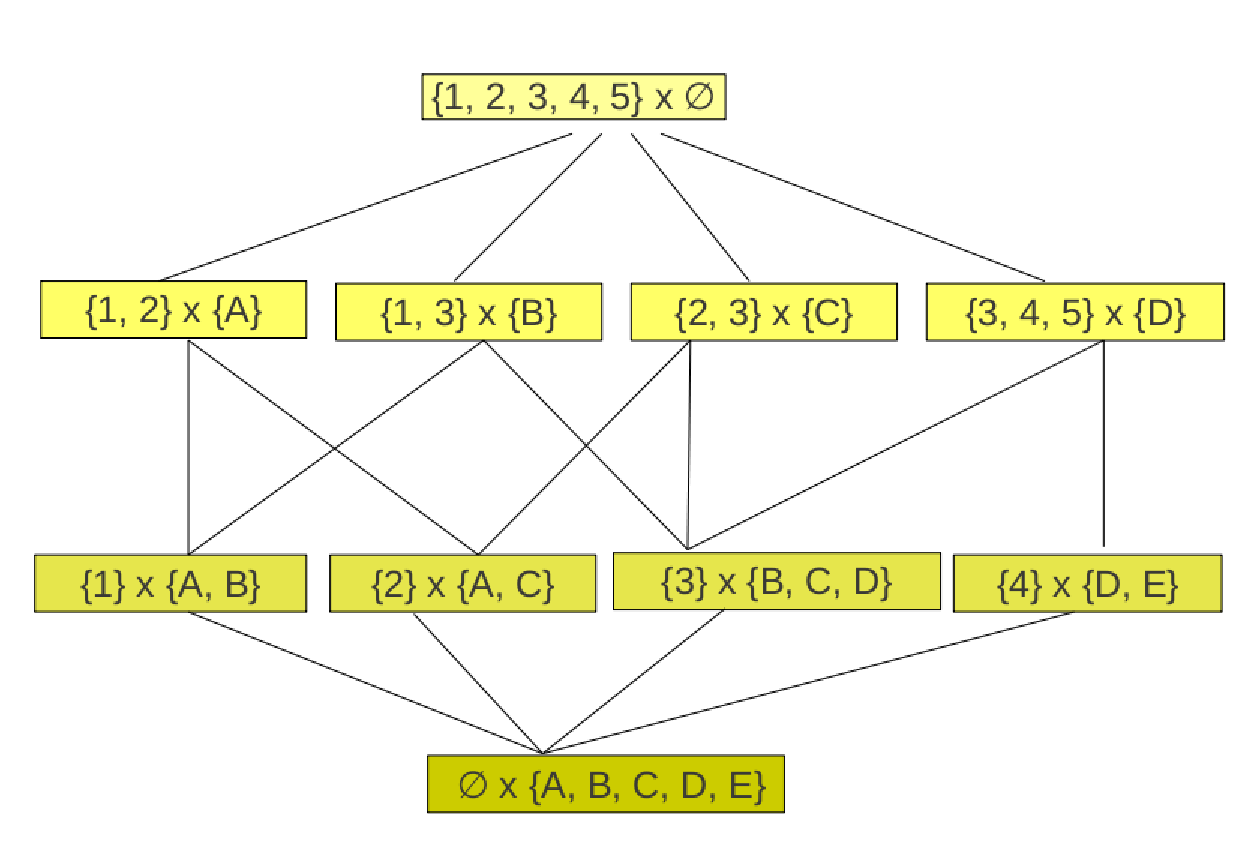
\includegraphics[width=7cm]{images/treillis}
\end{center}
\caption{ Treillis de Galois correspondant à  la table~\ref{ex_tab_0_1}}
\label{Fig:treillis}
\end{figure}

Il est  aisé d'en extraire un système de classes sur les individus en prenant les fermés de $h$, en y ajoutant les singletons et en enlevant l'ensemble vide. Ce qui est équivalent à considérer la fermeture par intersection non vide des colonnes de la table $T$ (les $Attr(j)$)  à qui on ajoute les singletons. 

Par exemple le système de classes associé à la table~\ref{ex_tab_0_1} est représenté dans la figure~\ref{Fig:treillis.moins}.

\begin{figure}
\begin{center}
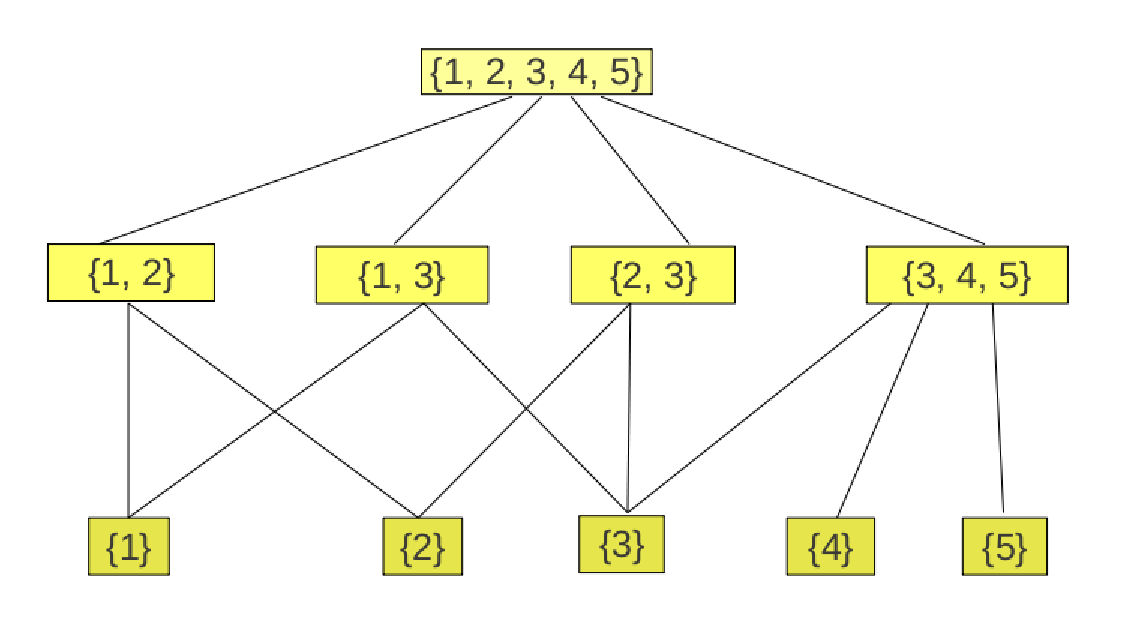
\includegraphics[width=7cm]{images/treillismoins}
\end{center}
\caption{ Système de classes correspondant à la table~\ref{ex_tab_0_1}}
\label{Fig:treillis.moins}
\end{figure}

\chapter{Structures démontables}
\label{structuredemonta}

Les treillis démontables permettent à la fois une analyse globale et locale des individus~:
\begin{itemize}
 \item L' analyse globale consiste dans le fait que ces treillis sont sans couronnes. Il sont aux treillis ce que sont les arbres pour les 
graphes~: une liaison minimale de structure pour les objets. Ils sont donc faciles à calculer et à représenter graphiquement puisque le nombre de leurs classes 
est borné par le carré du nombre des individus (voir~\cite{par_clu}).

 \item L'analyse locale consiste dans le fait qu'elles fournissent un ordre de démon\-tabilité selon un schéma d'élimination grâce auquel on trouve 
itérativement des éléments ``frontière'' de la structure~: les feuilles (définition~\ref{feuillesys}).

Ce schéma d'élimination se retrouve dans les trois structures~: Dans les treillis, il correspond à la suppression des éléments doublement irrédu\-ctibles
(section~\ref{doubleir}); dans les systèmes de classes, il correspond à la suppression d'individus (section~\ref{sysd}) ; et dans les tables 0/1, 
il correspond à la suppression de lignes (section~\ref{tdem}).

\end{itemize}

\label{structuresdemontables}

\section{Treillis démontable}
\label{doubleir}

\begin{definition}[\'Elément doublement irréductible ]


Pour un treillis $T = (E, \leq)$ muni des opérateurs sup ($\join$) et inf ($\meet$), on dit que $x \in E$ est: 
\begin{itemize}
 \item \textsc{Sup-irréductible}  si $\forall (x, y, z) \in E^3$, $x = y \join z \Rightarrow (x = y $ ou $ x = z)$
 \item \textsc{Inf-irréductible} si $\forall (x, y, z) \in E^3$, $x = y \meet z \Rightarrow (x = y$ ou $x = z)$
 \item \textsc{Doublement irréductible} s'il est sup-irréductible et inf-irréductible.
\end{itemize}

\end{definition}

\begin{definition}[Treillis démontable (Rival 1974)~\cite{rival1974}]

Un treillis $T = (E, \leq)$ est démontable s'il existe un élément doublement irréductible $x \in E$ tel que 
le treillis $T = (E \backslash \{x\}, \leq)$ reste démontable.
\end{definition}

Une conséquence quasi-directe de cette définition est de pouvoir remplacer le $\exists$ par un $\forall$. 
c'est-à-dire: 
$\forall x \in E$,
 $x$ est doublement irréductible $\Rightarrow$ $T = (E \backslash \{x\}, \leq)$ est un treillis démontable.

L'exemple illustré dans les figures~\ref{Fig:schema_elimination1_2} et~\ref{Fig:schema_elimination2_2} montre un schéma d'élimination des éléments d'un treillis démontable en  supprimant à chaque étape
 un élément doublement irréductible  du treillis restreint.

\begin{figure}
\begin{center}
\begin{tabular}{cc}
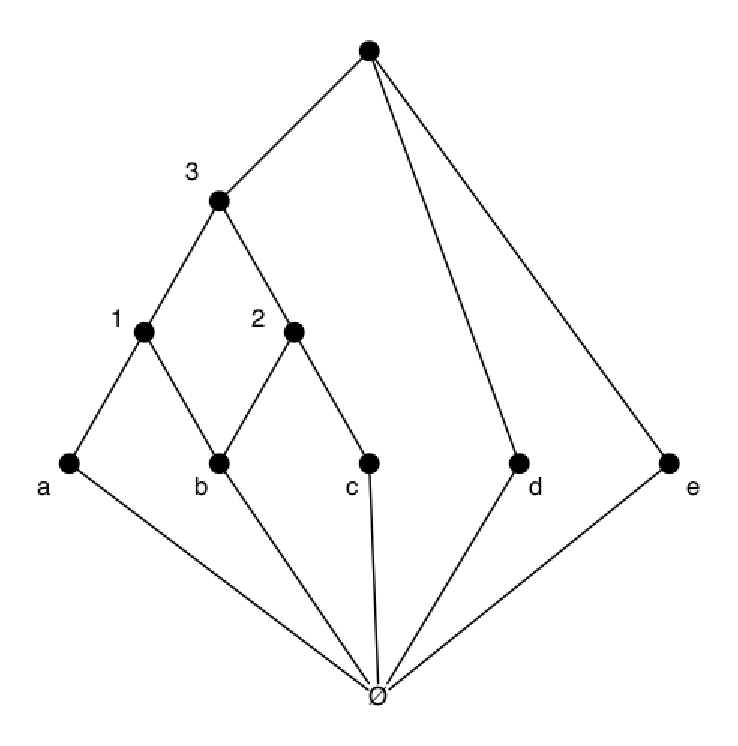
\includegraphics[scale=.5]{images/treillis1}&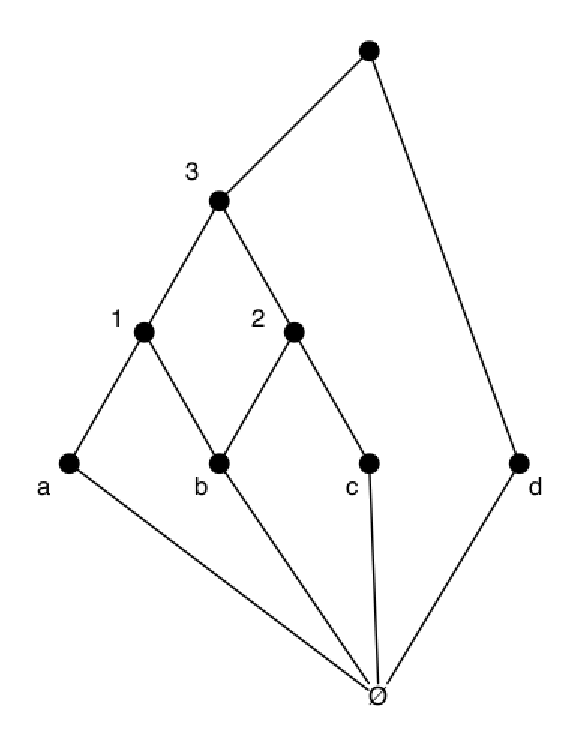
\includegraphics[scale=.5]{images/treillis2}\\
Treillis de départ & \'Elimination de la feuille e\\
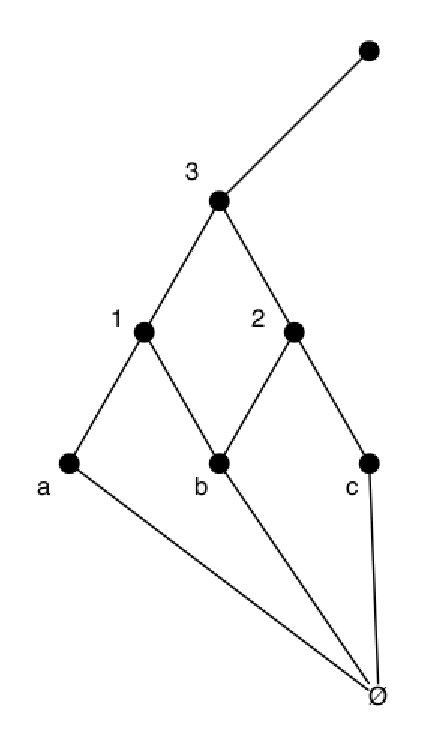
\includegraphics[scale=.5]{images/treillis3}&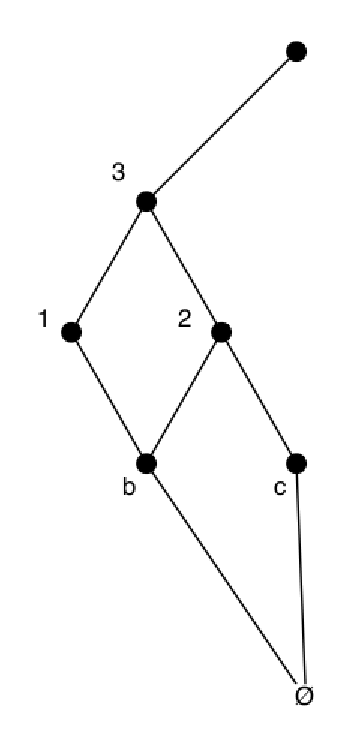
\includegraphics[scale=.5]{images/treillis4}\\
 \'Elimination de la feuille d & \'Elimination de la feuille a\\
\end{tabular}
\caption{Schéma d'élimination (1/2)~: feuilles initiales}
\label{Fig:schema_elimination1_2}
\end{center}
\end{figure}
\begin{figure}
\begin{center}
\begin{tabular}{cc}

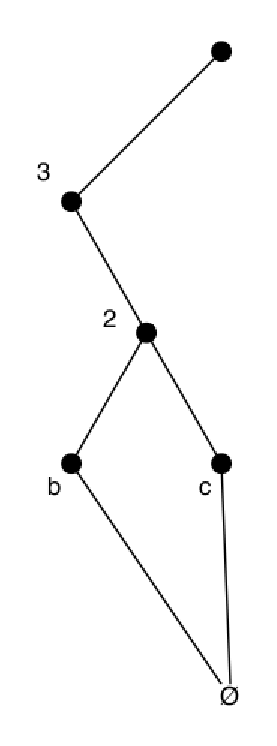
\includegraphics[scale=.5]{images/treillis5}&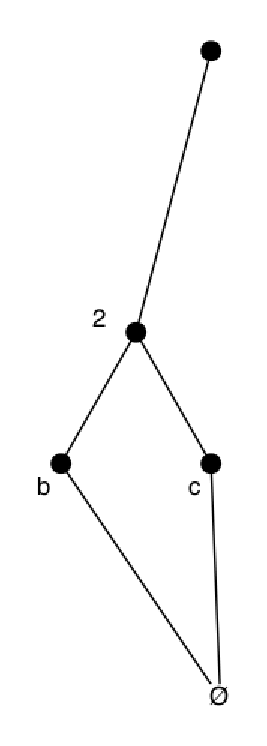
\includegraphics[scale=.5]{images/treillis6}\\
 \'Elimination de la feuille 1 & \'Elimination de la feuille 3\\
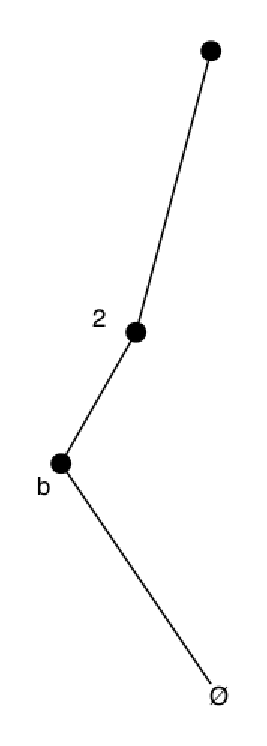
\includegraphics[scale=.5]{images/treillis7}&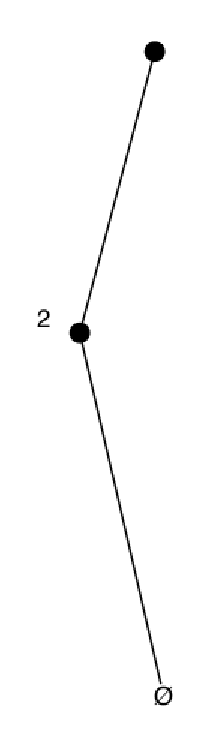
\includegraphics[scale=.5]{images/treillis8}\\
 \'Elimination de la feuille c & \'Elimination de la feuille b\\
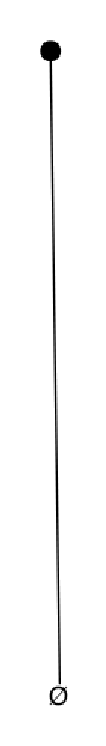
\includegraphics[scale=.5]{images/treillis9}&\\
\'Elimination de la feuille 2 &

\end{tabular}
\caption{Schéma d'élimination (2/2)~: feuilles suivantes}
\label{Fig:schema_elimination2_2}
\end{center}
\end{figure}

Cette définition par élimination successive est une propriété locale aux treillis démontables. Une propriété  globale consiste 
en l'absence de couronnes dans un treillis démontable (Théorème~\ref{treillisdemontable}).

\begin{definition}[Couronne]

Soit  $T = (E,\leq )$ un treillis. Une couronne est un ensemble partiellement ordonné $\{x_1, y_1,x_2, y_2,\ldots,x_n, y_n\}$ tel que:
\begin{itemize}
 \item  $x_n < y_n$ et $x_1 < y_n$,
 \item  $x_i < y_i $ et $ y_i > x_{i + 1}$ , pour $1 \leq i \leq n-1$
\end{itemize}

\end{definition}

La figure~\ref{fig:crown} illustre des exemples de couronnes.
\begin{figure}

\begin{center}

\begin{tabular}{c p{0.5cm} c}
\includegraphics[width=5cm]{images/3crown}  & &
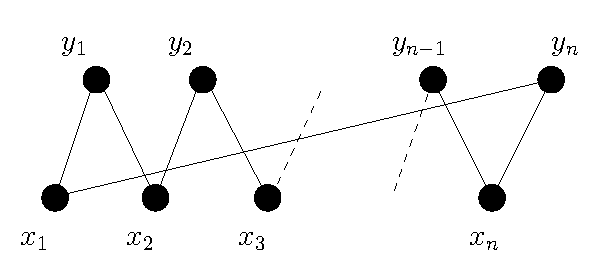
\includegraphics[width=5cm]{images/nCrown} \\
    $(a)$   & & $(b)$   \\
\end{tabular}

\end{center}
\caption{Exemples de couronnes}
\label{fig:crown}
\end{figure}

\begin{theorem}[Treillis démontable(Kelly et Rival 1974)~\cite{kelly-rival74}]

\label{treillisdemontable}
Un treillis est démontable s'il n'a pas de couronne.
\end{theorem}


S'il est clair, grâce à la propriété locale, que le treillis de départ de la figure~\ref{Fig:schema_elimination1_2} est démontable puisqu'on l'a démonté 
petit à petit dans les figures~\ref{Fig:schema_elimination1_2} et~\ref{Fig:schema_elimination2_2} ; c'est grâce à la propriété globale qu'on peut visuellement affirmer que le 
treillis de la figure~\ref{Fig:treillis.moins} n'est pas démontable. En effet, on peut remarquer l'existence d'une couronne sur ce treillis.
On peut montrer (\cite{crow_free}) que dans un treillis démontable, il existe toujours au moins un élément 
doublement irréductible dont le filtre est une chaîne.

\begin{definition}[chaîne]

\label{chaine}

Soit $\mathcal{R}$ une relation d'ordre sur un ensemble $E = \{e_1, e_2, \hdots ,e_n\}$.
On dit que les éléments de $E$ forment une \textsc{chaîne} pour la relation $\mathcal{R}$ si et seulement s'il existe une permutation $\sigma$ sur $[1..n]$
 telle que~:

$e_{\sigma(1)}~\mathcal{R}~e_{\sigma(2)}~\mathcal{R}~\hdots~\mathcal{R}~e_{\sigma(n-1)}~\mathcal{R}~e_{\sigma(n)}$.
\end{definition}

Dans la suite, on considère $\mathcal{R}$ comme l'opération inclusion $\subseteq$ sur les ensembles. On parlera alors de chaîne sur un ensemble sans 
préciser la relation d'ordre.

\begin{definition}[Filtre]

\label{filtre}
Soit un treillis $T = (E, \leq)$ et $i \in E$. Le filtre de $i$ noté $\uparrow i$ est défini par: $\uparrow i =\{i' \in E | i' \leq i \}$.
\end{definition}

Dans l'exemple du treillis de départ de la figure~\ref{Fig:schema_elimination1_2}, on a:
\begin{itemize}
\item $\uparrow a =\{a, ab, abc, abcde \}$,
\item $\uparrow b =\{ab, bc, abc, abcde \}$. 
\end{itemize}

L'Objet $a$ est une feuille car $a \subseteq ab \subseteq abc \subseteq abcde$. En revanche, 
$b$ n'est pas une feuille car $ab  \not\subseteq  bc$ et  $bc  \not\subseteq ab$.
 

\section{Système de classes démontable}

\label{sysd}

Le schéma d'élimination d'un treillis démontable peut \^etre transposé
aux systèmes de classes en supprimant du système de classes les \textsc{feuilles} (défini\-tion~\ref{feuillesys}) du treillis correspondant (\cite{par_clu}).
On rappelle les résultats obtenus dans ce domaine avant d'étendre cette propriété à la structure table 0/1 dans le dernier chapitre de  cet article.

\begin{proposition}[Système de classes restreint]

Soit $\mathcal{H} = (X, \mathcal{E})$ un sys\-tème de classes et $i \in X$,
Soit $\mathcal{E}^{'}$ construit comme suit~:

$\forall A \in \mathcal{E},$
\begin{itemize}
 \item $i \notin A \Rightarrow A \in \mathcal{E}^{'}$;
 \item $i \in A$ et $|A| > 1  \Rightarrow A \backslash \{i\}  \in \mathcal{E}^{'}$;
 \item Aucun autre ensemble n'appartient à $\mathcal{E}^{'}$.
\end{itemize}

Notons en plus~: $\mathcal{H} \backslash \{i\} = (X \backslash \{i\} , \mathcal{E}^{'})$

On a alors~: 
$(\mathcal{H} \backslash \{i\})$ est un système de classes.

\end{proposition}

\begin{definition}[Feuille sur un système de classes]

\label{feuillesys}

un élément $i \in X$ est une feuille sur un système de classes $F$ si son filtre  $\uparrow i$ forme une chaîne.
\end{definition}

Dans le système de classes de départ de la figure~\ref{sc_schema_elimination}, $a$ est une feuille car $\uparrow a$ est une chaîne
 puisque $\{a\} \subseteq \{a, b\} \subseteq \{a, b, c\} \subseteq \{a, b, c, d, e\}$.
Tandis que $b$ n'est pas une feuille car $\{a, b\}  \not\subseteq \{b, c\}$ et $\{c, b\}  \not\subseteq \{a, b\}$.


\begin{definition}[Système de classes démontable]

\label{sysclassdemontable}
Un système de classe $\mathcal{H}$ est démontable s'il contient une feuille $x$ tel que $\mathcal{H} \backslash \{x\}$ 
reste démontable.
\end{definition}

Notons également qu'un système de classes est démontable si et seulement si le treillis associé est démontable (\cite{par_clu}).

\begin{figure}
\begin{center}
\begin{tabular}{cc}
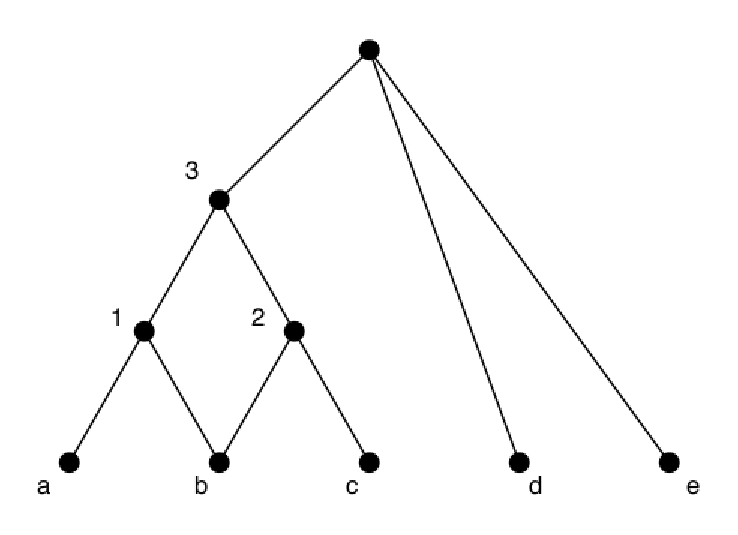
\includegraphics[scale=.5]{images/classes1}&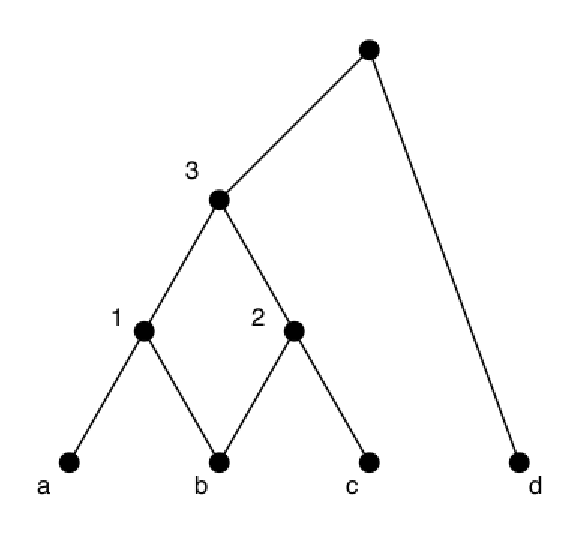
\includegraphics[scale=.5]{images/classes2}\\
Système de classes de départ &\'Elimination de la feuille e\\
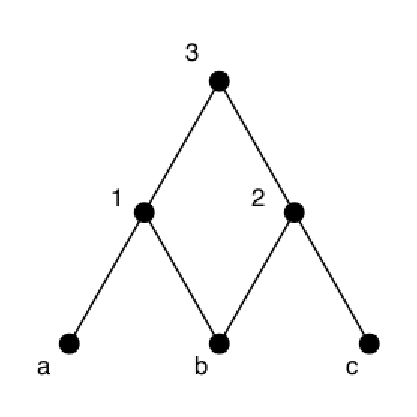
\includegraphics[scale=.5]{images/classes3}&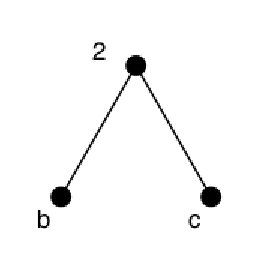
\includegraphics[scale=.5]{images/classes4}\\
\'Elimination de la feuille d &\'Elimination de la feuille a\\
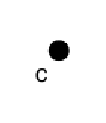
\includegraphics[scale=.5]{images/classes5}&\\
\'Elimination de la feuille b &
\end{tabular}
\caption{Système de classe~: schéma d'élimination}
\label{sc_schema_elimination}
\end{center}

\end{figure}
\chapter{Tables ordonnables}

\label{tdem}
Nous réutilisons les résultats de la partie précédente pour étendre la notion de démontabilité aux tables 0/1.
On introduit une propriété locale sur une table 0/1 caractérisant sa démontabilité. On met ainsi en relation 
les résultats obtenus sur les treillis démontables et les tables 0/1 ordonnables.\\
Cela nous permettra de donner un schéma d'élimination sur les tables et le mettre en bijection avec le schéma d'élimination sur les treillis
démontables.(section~\ref{sens1} et~\ref{sens2})

\begin{definition}[Configuration $\Gamma$]

\label{gamma}

Soit une table 0/1 $T$ définie par ses termes $T(i, j)$ où $1 \leq i \leq n$ et $1 \leq j \leq m$.
On appelle la configuration $\Gamma$ dans la table $T$ la configuration illustrée dans la table~\ref{gammma}.

c'est-à-dire~: 
pour tout $(i, j, j')$ tel que $1 \leq i \leq n$ et $1 \leq j < j' \leq m$,\\
Si $T_{(i, j')} = T_{(i, j)} = 1$ Alors $\forall i'\geqslant i, T_{(i', j)} = 1 \Rightarrow T_{(i', j')} = 1$.

\end{definition}

\begin{table}[htb]
\centering
 \begin{tabular}{*{4}{c|} c}
 
   $\cdots$ & $j$ & $\cdots$ & $j'$ & $\cdots$\\
 \hline
   $i$ & 1 & $\cdots$ & 1 & $\cdots$\\
 \hline
   $\cdots$ & * & $\cdots$ & * & $\cdots$\\
 \hline
   $i'$ & 1 & $\cdots$ & 0 & $\cdots$
 \end{tabular}
\caption{Configuration $\Gamma$}
\label{gammma}
\end{table}

\begin{definition}[Table bien ordonnée]

\label{demontable}

Une Table 0/1 qui ne contient pas de configuration $\Gamma$ (Cf définition~\ref{gamma}) est appelée
 table \textit{bien ordonnée}.
\end{definition}

\begin{definition}[Table ordonnable]

\label{tableordonnable}

Une Table 0/1 $T$ est \textit{ordonnable} si et seulement s'il existe une permutation $\sigma_L$ sur les lignes 
et une permutation $\sigma_C$ sur les colonnes telles que~:
la table $T'$ définie par $T'_{(i, j)} = T_{(\sigma_L(i), \sigma_C(j))}$ pour tout $(i, j)$ entiers naturels 
non nuls soit bien ordonnée.
\end{definition}

Par exemple la table~\ref{ex_tab_0_1} n'est pas bien ordonnée car elle contient au moins deux configurations $\Gamma$ (lignes $x_1$, $x_2$, colonnes $a_1$, $a_2$ ;
 et lignes $x_4$, $x_5$, colonnes $a_3$, $a_4$).

Cette table n'est de plus pas ordonnable. Permutons par exemple les lignes $x_1$ et $x_2$,
 puis les lignes $x_4$ et $x_5$ pour ne plus obtenir les deux configurations $\Gamma$ de la table~\ref{ex_tab_0_1}. 

\begin{table}[htb]
  \centering

\begin{tabular}{lccccc}
 & $a'_1$ & $a'_2$ & $a'_3$ & $a'_4$ & $a'_5$\\
$x'_1$ & \textbf{1} & \textbf{0} & \textbf{1} & \textbf{0} & \textbf{0}\\
$x'_2$ & \textbf{1} & \textbf{1} & \textbf{0} & \textbf{0} & \textbf{0}\\
$x'_3$ & \textbf{0} & \textbf{1} & \textbf{1} & \textbf{1} & \textbf{0}\\
$x'_4$ & \textbf{0} & \textbf{0} & \textbf{0} & \textbf{1} & \textbf{0}\\
$x'_5$ & \textbf{0} & \textbf{0} & \textbf{0} & \textbf{1} & \textbf{1}

\end{tabular}

\caption{Table~\ref{ex_tab_0_1} après permutations}

\label{3ex_tab_0_1}

\end{table}

Remarquons la nouvelle configuration $\Gamma$ sur les lignes $x'_1$ et $x'_2$. 
Nous laissons au lecteur le soin de tester toutes les autres permutations de lignes 
possibles mais une configuration $\Gamma$ apparaît à chaque fois (le treillis associé contient une couronne...).

Modifions légèrement la table~\ref{ex_tab_0_1} en posant par exemple $T_{(2,2)} = 1$ 

\begin{table}[htb]
  \centering

\begin{tabular}{lccccc}
 & $a''_1$ & $a''_2$ & $a''_3$ & $a''_4$ & $a''_5$\\
$x''_1$ & \textbf{1} & \textbf{1} & \textbf{0} & \textbf{0} & \textbf{0}\\
$x''_2$ & \textbf{1} & \textbf{1} & \textbf{1} & \textbf{0} & \textbf{0}\\
$x''_3$ & \textbf{0} & \textbf{1} & \textbf{1} & \textbf{1} & \textbf{0}\\
$x''_4$ & \textbf{0} & \textbf{0} & \textbf{0} & \textbf{1} & \textbf{1}\\
$x''_5$ & \textbf{0} & \textbf{0} & \textbf{0} & \textbf{1} & \textbf{0}
\end{tabular}

\caption{Table ~\ref{ex_tab_0_1} avec ajout d'un 1}

\label{12ex_tab_0_1}

\end{table}


Appliquons maintenant la permutation des lignes $x_4$ et $x_5$~:

\begin{table}[htb]
  \centering

\begin{tabular}{lccccc}
 & $a'''_1$ & $a'''_2$ & $a'''_3$ & $a'''_4$ & $a'''_5$\\
$x'''_1$ & \textbf{1} & \textbf{1} & \textbf{0} & \textbf{0} & \textbf{0}\\
$x'''_2$ & \textbf{1} & \textbf{1} & \textbf{1} & \textbf{0} & \textbf{0}\\
$x'''_3$ & \textbf{0} & \textbf{1} & \textbf{1} & \textbf{1} & \textbf{0}\\
$x'''_4$ & \textbf{0} & \textbf{0} & \textbf{0} & \textbf{1} & \textbf{0}\\
$x'''_5$ & \textbf{0} & \textbf{0} & \textbf{0} & \textbf{1} & \textbf{1}

\end{tabular}

\caption{Table~\ref{12ex_tab_0_1} après permutations}

\label{3ex_tab_0_1_dem}

\end{table}

Cette nouvelle table est bien ordonnée car elle ne contient aucune configuration $\Gamma$. La table~\ref{12ex_tab_0_1} est donc ordonnable. 
Dans le chapitre suivant, Nous allons démontrer qu'une table est ordonnable si et seulement si le treillis associé est démontable. 
Construisons le treillis associé à la table~\ref{12ex_tab_0_1} pour voir qu'il est effectivement démontable.
Commençons par trouver les fermés (table~\ref{tablefer}).
\begin{table}[htb]

\centering

\begin{tabular}{l|c|c|c}

$A$ & $g(A)$ & $h(A)$ & $A = h(A) ?$\\
\hline
$a'''_1$ & $x'''_1x'''_2$ & $a'''_1a'''_2$ & \\
\hline
\textbf{$a'''_1a'''_2$} & \textbf{$x'''_1x'''_2$} & $a'''_1a'''_2$ & $\surd$\\
\hline
$a'''_1a'''_3$ &$x'''_2$ & $a'''_1a'''_2a'''_3$ & \\
\hline
$a'''_1a'''_4$ & $\varnothing$ & $a'''_1a'''_2a'''_3a'''_4a'''_5$ & \\
\hline
$a'''_1a'''_5$ & $\varnothing$ & $a'''_1a'''_2a'''_3a'''_4a'''_5$ & \\
\hline
\textbf{$a'''_1a'''_2a'''_3$} & \textbf{$x'''_2$} & $a'''_1a'''_2a'''_3$ & $\surd$\\
\hline
$a'''_1a'''_2a'''_4$ & $\varnothing$ & $a'''_1a'''_2a'''_3a'''_4a'''_5$ & \\
\hline
$a'''_1a'''_2a'''_5$ & $\varnothing$ & $a'''_1a'''_2a'''_3a'''_4a'''_5$ & \\
\hline
$a'''_1a'''_3a'''_4$ & $\varnothing$ & $a'''_1a'''_2a'''_3a'''_4a'''_5$ & \\
\hline
$a'''_1a'''_3a'''_5$ & $\varnothing$ & $a'''_1a'''_2a'''_3a'''_4a'''_5$ & \\
\hline
$a'''_1a'''_4a'''_5$ & $\varnothing$ & $a'''_1a'''_2a'''_3a'''_4a'''_5$ & \\
\hline
$a'''_1a'''_2a'''_3a'''_4$ & $\varnothing$ & $a'''_1a'''_2a'''_3a'''_4a'''_5$ & \\
\hline
$a'''_1a'''_2a'''_3a'''_5$ & $\varnothing$ & $a'''_1a'''_2a'''_3a'''_4a'''_5$ & \\
\hline
$a'''_1a'''_3a'''_4a'''_5$ & $\varnothing$ & $a'''_1a'''_2a'''_3a'''_4a'''_5$ & \\
\hline
\textbf{$a'''_1a'''_2a'''_3a'''_4a'''_5$} & \textbf{$\varnothing$} & $a'''_1a'''_2a'''_3a'''_4a'''_5$ & $\surd$\\
\hline
\textbf{$a'''_2$} & \textbf{$x'''_1x'''_2x'''_3$} & $a'''_2$ & $\surd$\\
\hline
\textbf{$a'''_2a'''_3$} & \textbf{$x'''_2x'''_3$} & $a'''_2a'''_3$ & $\surd$\\
\hline
$a'''_2a'''_4$ & $x'''_3$ & $a'''_2a'''_3a'''_4$ & \\
\hline
$a'''_2a'''_5$ & $\varnothing$ & $a'''_1a'''_2a'''_3a'''_4a'''_5$ & \\
\hline
\textbf{$a'''_2a'''_3a'''_4$} & \textbf{$x'''_3$} & $a'''_2a'''_3a'''_4$ & $\surd$\\
\hline
$a'''_2a'''_3a'''_5$ & $\varnothing$ & $a'''_1a'''_2a'''_3a'''_4a'''_5$ & \\
\hline
$a'''_2a'''_4a'''_5$ & $\varnothing$ & $a'''_1a'''_2a'''_3a'''_4a'''_5$ & \\
\hline
$a'''_2a'''_3a'''_4a'''_5$ & $\varnothing$ & $a'''_1a'''_2a'''_3a'''_4a'''_5$ & \\
\hline
$a'''_3$ & $x'''_2x'''_3$ & $a'''_2a'''_3$ & \\
\hline
$a'''_3a'''_4$ & $x'''_3$ & $a'''_2a'''_3a'''_4$ & \\
\hline
$a'''_3a'''_5$ & $\varnothing$ & $a'''_1a'''_2a'''_3a'''_4a'''_5$ & \\
\hline
$a'''_3a'''_4a'''_5$ & $\varnothing$ & $a'''_1a'''_2a'''_3a'''_4a'''_5$ & \\
\hline
\textbf{$a'''_4$} & \textbf{$x'''_3x'''_4x'''_5$} & $a'''_4$ & $\surd$\\
\hline
\textbf{$a'''_4a'''_5$} & \textbf{$x'''_5$} & $a'''_4a'''_5$ & $\surd$\\
\hline
$a'''_5$ & $x'''_5$ & $a'''_4a'''_5$ & \\
\hline
\textbf{$\varnothing$} & \textbf{$a'''_1a'''_2a'''_3a'''_4a'''_5$} & $\varnothing$ & $\surd$

\end{tabular}

\caption{Les fermés de la table~\ref{3ex_tab_0_1_dem}}
\label{tablefer}
\end{table}
Le treillis associé est illustré dans la figure~\ref{figure_treillis_associe}.
\begin{figure}
\begin{center}
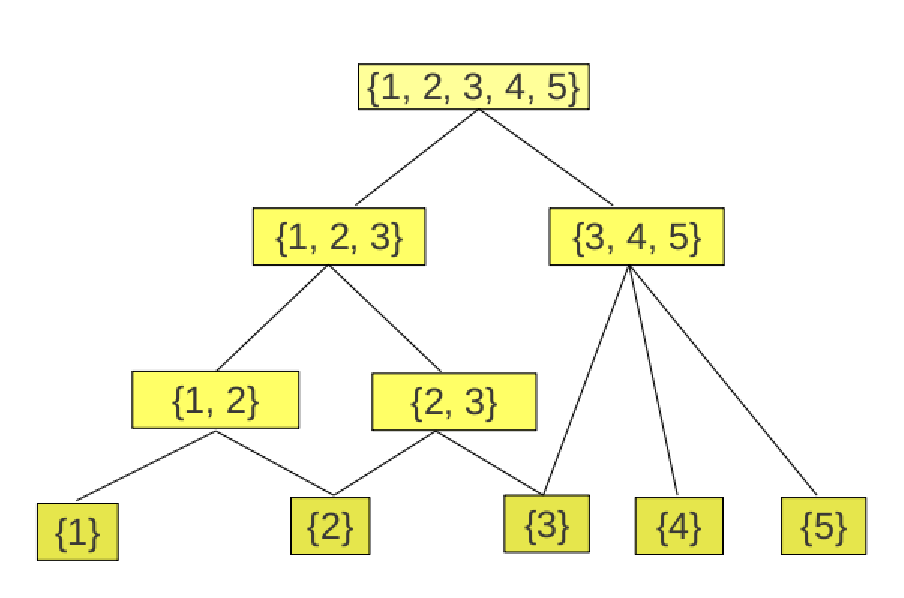
\includegraphics[width=7cm]{images/treillismoins2}
\end{center}
\caption{ Système de classes associé à la table~\ref{3ex_tab_0_1_dem}.}
\label{figure_treillis_associe}
\end{figure}
Ce treillis est démontable car il ne contient pas de couronne (la classe \{1, 3\} du treillis de la figure~\ref{Fig:treillis.moins} a été transformée en la classe \{1, 2, 3\}).

\chapter{Tables 0/1 démontables}

Dans ce chapitre, on s'appuie sur la structure système de classes pour étendre la bijection entre le treillis et le système de classes aux tables 0/1.
\label{results}

\section{Feuilles}

On commence par étendre la notion de feuille à la structure table 0/1 puis on établie la bijection avec la notion de feuille sur un système de classes. 
Ceci nous permettra de fabriquer un schéma d'élimination sur les tables 0/1 (section~\ref{sens1}). On démontre ensuite qu'une table est ordonnable 
si et seulement si le système de classes associé est démontable (section~\ref{sens2}).
\begin{definition}[Feuille sur une table 0/1]

\label{feuilletable}

Un individu $x_i$ est une feuille sur une table 0/1 $T$ si ses classes s'emboitent.

C'est-à-dire~:
$\forall (a_j, a_j') \in Attr(x_i)^2, Ind(a_j) \subseteq Ind(a_j')$ ou $Ind(a_j') \subseteq Ind(a_j)$.

\end{definition}

\begin{proposition}

\label{lemmedetravail}

Une table 0/1 $T$ est bien ordonnée( Cf définition~\ref{demontable} )
si et seulement si, 
pour tout $(i, x_{i_0}, a_j, a_{j'})$ tels que: $1 \leq a_j < a_{j'} \leq m$ et $1 \leq x_{i_0} \leq i \leq n$
\begin{equation}
x_{i_0} \in Ind_{}(a_j) \cap Ind_{}(a_{j'}) 
\Rightarrow
 Ind_{\geqslant x_{i_0}}(a_j) \subseteq Ind_{\geqslant x_{i_0}}(a_{j'})
\label{hyp} 
\end{equation}
\end{proposition}

\begin{table}[htb]
\centering
 \begin{tabular}{*{7}{c|} c}
  %\backslashbox{Individu}{Classe}
     & $\cdots$ & $a_j$ & $\cdots$ & $a_{j'}$  & $\cdots$ & $a_{j'}'$ & $\cdots$\\
 \hline
   $i$ & $\cdots$ & $///$ & $\cdots$ & $///$  & $\cdots$ & $///$  & $\cdots$\\
 \hline
  $\vdots$ & $\vdots$ & $\vdots$ & $\vdots$ & $\vdots$  & $\vdots$ & $\vdots$ & $\vdots$\\
 \hline
   $x_{i_0}$ & $\cdots$ & 1 & $\cdots$ & 1 & $\cdots$ & 1 & $\cdots$\\
 \hline
   $x_{i_0} + 1$ & $\cdots$ & 0 & $\cdots$ & 1 & $\cdots$ & 1 & $\cdots$\\
 \hline
   $x_{i_0} + 2$ & $\cdots$ & 0 & $\cdots$ & 0 & $\cdots$ & 1 & $\cdots$\\
 \hline
   $x_{i_0} + 3$ & $\cdots$ & 1 & $\cdots$ & 1 & $\cdots$ & 1 & $\cdots$\\
 \end{tabular}
\caption{Illustration de l'équation~\ref{hyp}}
\end{table}


\begin{preuve}

\paragraph{$(\Rightarrow)$}
Supposons $(x_{i_0}, a_j, a_{j'})$ tels que~: $1 \leq a_j < a_{j'} \leq m$ et $T_{(x_{i_0}, a_{j'})} = T_{(x_{i_0}, a_j)} = 1$.
Supposons de plus qu'il existe $x_{i'}$ tel que:  $n \geqslant x_{i'}\geqslant x_{i_0} \geqslant 1$ et $T_{(x_{i'}, a_j)} = 1$.
Si $T_{(x_{i'}, a_{j'})} = 0$,
alors la table 0/1 contient la configuration $\Gamma$ (définition~\ref{gamma})~:
\begin{table}[htb]
\centering
 \begin{tabular}{*{4}{c|} c}
   $\cdots$ & $a_j$ & $\cdots$ & $a_{j'}$ & $\cdots$\\
 \hline   
   $i<x_{i_0}$ & $///$ & $\cdots$ & $///$ & $\cdots$\\
 \hline
   $x_{i_0}$ & 1 & $\cdots$ & 1 & $\cdots$\\
 \hline
   $\cdots$ & * & $\cdots$ & * & $\cdots$\\
 \hline
   $x_{i'}$ & 1 & $\cdots$ & 0 & $\cdots$
 \end{tabular}
\caption{Configuration $\Gamma$ de la table $T$}
\end{table}

Ce qui contredit le fait que la table $T$ soit bien ordonnée.
Donc $T_{(x_{i'}, a_{j'})} = 1$, 
d'où $Ind_{\geqslant x_{i_0}}(a_j) \subseteq Ind_{\geqslant x_{i_0}}(a_{j'})$.

\paragraph{$(\Leftarrow)$}
Soit $(x_{i_0}, a_j, a_{j'})$ tel que~:

 $1 \leq a_j < a_{j'} \leq m$ et $1 \leq x_{i_0} \leq n$ et $T_{(x_{i_0}, a_j)} = T_{(x_{i_0}, a_{j'})} =1$.

Montrons alors que la table T est bien ordonnée (définition~\ref{demontable})~:  
Supposons qu'il existe $x_{i'}$ tel que $1 \leq x_{i_0} \leq x_{i'} \leq n$ et $T_{(x_{i'}, j)} =1$.
Si $T_{(x_{i'}, a_{j'})} = 0$
alors 
$Ind_{\geqslant x_{i_0}}(a_j)  \not\subseteq Ind_{\geqslant x_{i_0}}(a_{j'})$
Or, $x_{i_0} \in Ind_{}(a_j) \cap Ind_{}(a_{j'})$  (car $T_{(x_{i_0}, a_j)} = T_{(x_{i_0}, a_{j'})} = 1$). 
Donc d'après l'hypothèse (\ref{hyp}): $Ind_{\geqslant x_{i_0}}(a_j) \subseteq Ind_{\geqslant x_{i_0}}(a_{j'})$. 
Donc $T_{(x_{i'}, a_{j'})} = 1$ et la table $T$ est bien ordonnée.
\begin{table}[htb]
  \centering

 \begin{tabular}{*{4}{c|} c}
   $\cdots$ & $a_j$ & $\cdots$ & $a_{j'}$ & $\cdots$\\
 \hline   
   $k<x_{i_0}$ & $///$ & $\cdots$ & $///$ & $\cdots$\\
 \hline
   $x_{i_0}$ & 1 & $\cdots$ & 1 & $\cdots$\\
 \hline
   $\cdots$ & * & $\cdots$ & * & $\cdots$\\
 \hline
   $x_{i'}$ & 1 & $\cdots$ & 0 & $\cdots$
 \end{tabular}
\caption{Cas où  $T_{(x_{i'}, a_{j'})} = 0$ }
\end{table}

$\Box$
\end{preuve}

\paragraph{}Par exemple, dans la table bien ordonnée~\ref{3ex_tab_0_1_dem} on a~:

$x'''_3\in Ind_{\geqslant x'''_3}(a'''_2) \cap Ind_{\geqslant x'''_4}(a'''_4)$ 
 et $Ind_{\geqslant x'''_3}(a'''_2) \subseteq Ind_{\geqslant x'''_3}(a'''_4)$.

Reste à montrer l'équivalence entre une feuille sur une table 0/1 et son système de classes associé. C'est l'objet de la proposition~\ref{propfeuille}.

\begin{proposition}[Correspondance des feuilles]
\label{propfeuille}
Soit $F$ le système de classes associé à une table 0/1 $T$.

$x_i$ est une feuille sur $F$ (Cf définition~\ref{feuillesys})
$\Leftrightarrow$
$x_i$ est une feuille sur la table 0/1 $T$ (Cf définition~\ref{feuilletable}).
\end{proposition}

\begin{preuve}


\paragraph{$(\Rightarrow)$}
Supposons $i$ une feuille sur $F$, alors $\uparrow i$ forme une chaîne. 
Donc, $\exists p > 0$ tel que $\uparrow i = \{S_1, S_2,..., S_p\}$ avec
\begin{equation}
\label{inclusion}
 S_1 \subseteq S_2 \subseteq ... \subseteq S_p.
\end{equation}
Soit $(j, j') \in Attr(i)^2$. 
Alors,
$\exists k_1$ tel que  $1 \leqslant k_1 \leqslant p$ et $Ind(j) = S_{k_1}$
et
$\exists k_2$ tel que  $1 \leqslant k_2 \leqslant p$ et $Ind(j') = S_{k_2}$.
Donc d'après la relation~\ref{inclusion}, $Ind(j) \subseteq Ind(j')$ ou $Ind(j') \subseteq Ind(j)$. D'où $i$ est feuille sur $T$.

\paragraph{$(\Leftarrow)$}
Supposons $i$ une feuille sur la table 0/1 $T$. 
Alors, $\forall (j, j') \in Attr(i), Ind(j) \subseteq Ind(j')$ ou $Ind(j') \subseteq Ind(j)$. 
Donc, $\exists l > 0$ tel que $Attr(i) = \{j_1, j_2,..., j_l\}$  avec
\begin{equation}
\label{inclusion2}
 Ind(j_1) \subseteq Ind(j_2) \subseteq ... \subseteq Ind(j_l).
\end{equation}
Comme l'ensemble des classes $F$ est la fermeture par intersection 
des $Ind(j_k)$ pour $1 \leqslant k \leqslant l$, 
pour tout $S \in F$ avec $i \in S$, il existe $L \subseteq \{1...l\}$ tel que~:
 $S = \bigcap_{k \in L} Ind(j_k) = C_{min_{\subseteq}(L)}$ 
(grâce à la relation~\ref{inclusion2}). 
Les classes sont donc incluses les unes dans les autres en gardant l'ordre de la relation~\ref{inclusion2}.
D'où les éléments de $\uparrow i$ forment une chaîne et $i$ est une feuille sur $F$.

$\Box$
\end{preuve}

Par exemple, $x'''_1$ est une feuille sur la table~\ref{3ex_tab_0_1_dem} car $Attr(x'''_1) =\{a'''_1, a'''_2\}$ et  $a'''_2$ contient $a'''_1$ ; 
et $x'''_1$ est une feuille sur le treillis associé (figure~\ref{figure_treillis_associe}) car son filtre forme une chaîne.

\section{Ordonnabilité $\Rightarrow$ Démontabilité}

\label{sens2}


\begin{proposition}[Ordonnabilité - Démontabilité]

\label{tabletreillis}
Soit $\mathcal{H}$ le système de classes associé à une table présence/absence $T$.

$T$ est ordonnable (Cf définition~\ref{tableordonnable}) $\Rightarrow$ $\mathcal{H}$ est démontable. 

\end{proposition}

\begin{preuve}

Récurrence sur $n$: nombre de lignes de $T$.

Pour $n = 1$  la propriété est vraie (le treillis est réduit à un unique élément).
Supposons la propriété vraie pour le rang $n$ et considérons une table 0/1 $T'$ à $n + 1$ lignes qui est ordonnable.

Soit $T''$ la table ordonnée après ordonnancement de $T'$ (Cf définition~\ref{tableordonnable}).
La première ligne $l_1$ de $T''$ est une feuille sur la table $T''$ car ses classes s'emboîtent. 
Comme le système de classes associé à $T''$ est exactement celui associé à $T$, et 
d'après la proposition~\ref{propfeuille}, on a $l_1$ est une feuille sur le système de classes $\mathcal{H}$.

Soit $T^{\star}$ la table $T''$ privée de sa première ligne $l_1$.
$T^{\star}$ est ordonnée car $T''$ est ordonnée.
Or le système de classes  $\mathcal{H}^{\star}$ associé à $T^{\star}$ est exactement le système de 
classes $\mathcal{H}$ associé à $T$ restreint à $X \backslash \{l_1\}$ (Cf proposition~\ref{tablerestreinte}).
De plus $T^{\star}$ a exactement $n$ lignes, donc d'après l'hypothèse de
récurrence, $\mathcal{H}^{\star}$ est démontable.

Conclusion~:
\begin{itemize}
 \item Le système de classes $\mathcal{H}^{\star}$ associé à $T''$  est démontable. 
 \item $l_1$ est feuille sur $\mathcal{H}$. (car  $l_1$ est une feuille sur le système de classes $\mathcal{H}$)
\end{itemize}
Donc~: $\mathcal{H}$ est démontable.

$\Box$
\end{preuve}

\section{Démontabilité $\Rightarrow$ Ordonnabilité}

\label{sens1}

\begin{proposition}[Table restreinte]
\label{tablerestreinte}

Soit $\mathcal{H} = (X, \mathcal{E})$ le système de classes associé à une table 0/1 $T$.
Soit $T^{\star}$ la table $T$ privée de sa ligne $i$.
Soit $\mathcal{H}^{\star}$ le système de classes associé à $T^{\star}$.
On a alors~: 
$\mathcal{H}^{\star} = \mathcal{H} \backslash \{x_i\}  =(X \backslash \{x_i\} , \mathcal{E}^{'})$.

\end{proposition}

\begin{preuve}

\begin{center}
$T \Longleftrightarrow  \mathcal{H} = (X  , \mathcal{E})$

$\downarrow$ 

$T^{\star}  \Longleftrightarrow \mathcal{H}^{\star} = (X' , \mathcal{E}^{\star})$
\end{center}

\begin{itemize}
 \item montrons que $X' = X \backslash \{i\}$.
    \begin{itemize}
    \item 
$x \in X'
\Rightarrow
x$ est une ligne de $T^{\star}
\Rightarrow
x \in X \backslash \{i\}
$. 
    \item 
$x \in X \backslash \{i\}
\Rightarrow
x$ est une ligne de $T^{\star}
\Rightarrow
x \in X'
$. 
    \end{itemize}

 \item montrons que $\mathcal{E}^{\star} = \mathcal{E}^{'}$.
    \begin{itemize}
    \item
$A \in \mathcal{E}^{\star}
\Rightarrow
\exists X$ colonne de $T^{\star}$ tel que $A = g(X)$ et $i \notin g(X)
\Rightarrow
g(X) \in \mathcal{E}^{'}$ (par construction de $\mathcal{E}^{'}$)
$\Rightarrow
A \in \mathcal{E}^{'}
$
    \item 
Soit $A \in \mathcal{E}^{'}$, alors $i \notin A$ et on a deux cas~:
          \begin{itemize}
          \item $A \in \mathcal{E}$.
          Donc, il existe $X$ colonne de $T$ tel que $A = g(X)$.
          D'où, en considérant $X$ comme colonne de $T'$, il existe $X$ colonne de $T'$ tel que $A = g(X)$ et $i \notin A$.
          D'où $A \in \mathcal{E}^{\star}$

          \item $A \cup \{i\} \in \mathcal{E}.$
          Donc, il existe $X$ colonne de $T$ tel que $A \cup \{i\} = g(X)$.
          D'où, en enlevant $i$ à $T$, et en considérant $X$ comme colonne de $T^{\star}$, 
          on a $i \notin g(X)$ et $g(X) = (A \cup \{i\}) \backslash \{i\} = A$.
          D'où $A \in \mathcal{E}^{\star}$.
          \end{itemize}
    \end{itemize}
\end{itemize}

$\Box$
\end{preuve}

Commençons par énoncer l'algorithme qui aidera à démontrer cette propriété et appliquons le au cas de la table associée au système de classe de départ de
la figure~\ref{sc_schema_elimination}.

Considérons donc l'algorithme suivant~:

\begin{enumerate}
\item $find\_order(\mathcal{H});$ trouver un ordre de démontage des individus de $\mathcal{H}$. (le premier à être démonté est $x_n$ et le dernier $x_1$).
\item $T' = lignes\_reorder(T);$ ordonner les lignes de la table $T$ dans l'ordre de démontabilité de $\mathcal{H}$ (la première ligne est $x_1$ et la dernière est $x_n$).
\item
  \begin{itemize}
	\item Soit la fonction  $colonnes\_reorder$ qui prend en entrée une table $Tab$ de $n$ lignes et $m$ colonnes, et une ligne $x_k$ comprise entre $x_1$ et $x_n$ ; et qui retourne
 une table $Result$.

		  $colonnes\_reorder(Tab, x_k)$
		  \begin{itemize}
		   \item $Result = Tab;$
		   \item $D =$ table dont des lignes sont ceux de $Result$ dans leur ordre et les colonnes sont les $Attr(x_k)$.
		   \item $G =$ table dont des lignes sont ceux de $Result$ dans leur ordre et les colonnes sont les attribut $a$ tel que $a \notin Attr(x_k)$.
		   \item Si $|G.colonnes| > 1$ et $k > 1$, alors $colonnes\_reorder(G, x_{k-1});$
		   \item Si $|D.colonnes| > 1$ et $k > 1$, alors $colonnes\_reorder(D, x_{k-1});$
           \item $Result = concatenate (G, D);$ concaténation des tables $G$ et $D$ dans cet ordre.
		  \end{itemize}
		  $return$~$Result;$
  \end{itemize}
\item $TableOrdonnee = colonnes\_reorder(T', x_n);$
\end{enumerate}


Appliquons cet algorithme sur le système de classes démontable de la figure~\ref{figure_treillis_associe}. On sait que la table~\ref{3ex_tab_0_1_dem} lui est associée.

On peut démonter le système de classes en enlevant d'abord $x'''_5$, puis $x'''_4$, puis $x'''_3$, puis $x'''_2$, puis $x'''_1$. On réordonne les lignes et 
obtient alors la table~\ref{tablereor}.
 

\begin{table}[htb]
  \centering

\begin{tabular}{lccccc}
 & $a'''_1$ & $a'''_2$ & $a'''_3$ & $a'''_4$ & $a'''_5$\\
$x'''_1$ & \textbf{1} & \textbf{1} & \textbf{0} & \textbf{0} & \textbf{0}\\
$x'''_2$ & \textbf{1} & \textbf{1} & \textbf{1} & \textbf{0} & \textbf{0}\\
$x'''_3$ & \textbf{0} & \textbf{1} & \textbf{1} & \textbf{1} & \textbf{0}\\
$x'''_4$ & \textbf{0} & \textbf{0} & \textbf{0} & \textbf{1} & \textbf{0}\\
$x'''_5$ & \textbf{0} & \textbf{0} & \textbf{0} & \textbf{1} & \textbf{1}

\end{tabular}

\caption{Table~\ref{3ex_tab_0_1_dem} après réordonnement des lignes (elle ne change pas !)}
\label{tablereor}
\end{table}

On applique la fonction $colonnes\_reorder$ à la table~\ref{tablereor} pour obtenir la table~\ref{tablereor1}.

\begin{table}[htb]
  \centering

\begin{tabular}{lccccc}
 & $a'''_1$ & $a'''_3$ & $a'''_2$ & $a'''_5$ & $a'''_4$\\
$x'''_1$ & \textbf{1} & \textbf{0} & \textbf{1} & \textbf{0} & \textbf{0}\\
$x'''_2$ & \textbf{1} & \textbf{1} & \textbf{1} & \textbf{0} & \textbf{0}\\
$x'''_3$ & \textbf{0} & \textbf{1} & \textbf{1} & \textbf{0} & \textbf{1}\\
$x'''_4$ & \textbf{0} & \textbf{0} & \textbf{0} & \textbf{0} & \textbf{1}\\
$x'''_5$ & \textbf{0} & \textbf{0} & \textbf{0} & \textbf{1} & \textbf{1}

\end{tabular}

\caption{$colonnes\_reorder ($Table~\ref{tablereor}, $x'''_5)$}
\label{tablereor1}
\end{table}

Remarquons alors que la table~\ref{tablereor1} ne contient aucune configuration $\Gamma$. Elle est donc bien ordonnée, d'où 
la table associée au système de classes démontable de la figure~\ref{figure_treillis_associe} est ordonnable.

\begin{proposition}[Démontabilité - Ordonnabilité]

\label{tabletreillis2}
Soit $\mathcal{H}$ le système de classes associé à une table présence/absence $T$.

$\mathcal{H}$ est démontable $\Rightarrow$ $T$ est ordonnable (Cf définition~\ref{tableordonnable}) .  

\end{proposition}

\begin{preuve}

Supposons que $\mathcal{H}$ soit démontable, on sait alors qu'il existe un ordre de démontabilité des individus.
Il existe donc $n$ et $(x_i)_{1 \leqslant i \leqslant n}$ 
qui sont classés dans  un ordre de dèmontabilité.

Soit $T'$ la table $T$ avec réordonnancement des lignes dans l'ordre de démonta\-bilité de $\mathcal{H}$. 
Nous allons construire $T''$ en réordonnant les colonnes de $T'$.

On sait que les lignes de $T'$ sont formées des $(x_i)_{1 \leqslant i \leqslant n}$ dans leur ordre de 
démontabilité dans le système de classes $\mathcal{H}$.

\begin{table}[htb]
\centering
\begin{tabular}{ |c | c | c |c | c |}
\hline
 & $j_1$ & $j_2$ & $\cdots$ & $j_m$\\
\hline
$x_1$ & * & * & $\cdots$ & *\\
\hline
$x_2$ & * & * & $\cdots$ & *\\
\hline
$\vdots$ & $\vdots$ & $\vdots$ & $\cdots$ & $\vdots$\\
\hline
$x_i$ & * & * & $\cdots$ & *\\
\hline
$\vdots$ & $\vdots$ & $\vdots$ & $\cdots$ & $\vdots$\\
\hline
$\vdots$ & $\vdots$ & $\vdots$ & $\cdots$ & $\vdots$\\
\hline
$x_n$ & * & * & $\cdots$ & *\\
\hline
\end{tabular}
\caption{Table $T'$}
\end{table}


\'Etape 1~:

On sépare les colonnes en 2~: à gauche celles qui ne contiennent pas $x_n$~: $G$ et à droite celles qui le 
contiennent~: $D$.
On remarque qu'une colonne de $G$ ne peut inclure strictement une colonne de $D$.

\begin{table}[htb]
 \centering

\begin{tabular}{ |c | c | c |c | c | c | c | c |c |}
\hline
 & $j_{\sigma_{C}^{1}(1)}$ & $j_{\sigma_{C}^{1}(2)}$ & $j_{\sigma_{C}^{1}(3)}$ & $\cdots$  & $j_{\sigma_{C}^{1}(j_{m - 3})}$ & $j_{\sigma_{C}^{1}(j_{m - 2})}$ & $j_{\sigma_{C}^{1}(j_{m - 1})}$ & $j_{\sigma_{C}^{1}(j_{m})}$\\
\hline
$x_1$ & * & * & * & $\cdots$ & * & * & * & *\\
\hline
$x_2$ & * & * & * & $\cdots$ & * & * & * & *\\
\hline
$\vdots$ & $\vdots$ & $\vdots$ & $\vdots$ & $\cdots$ & $\vdots$ & $\vdots$ & $\vdots$ & $\vdots$\\
\hline
$\vdots$ & $\vdots$ & $\vdots$ & $\vdots$ & $\cdots$ & $\vdots$ & $\vdots$ & $\vdots$ & $\vdots$\\
\hline
$\vdots$ & $\vdots$ & $\vdots$ & $\vdots$ & $\cdots$ & $\vdots$ & $\vdots$ & $\vdots$ & $\vdots$\\
\hline
$x_{n-1}$ & * & * & * & $\cdots$ & * & * & * & *\\
\hline
$x_n$ & $0$ & $0$ & $0$ & $\cdots$ & $1$ & $1$ & $1$ & $1$\\
\hline
\end{tabular}
\caption{Table $T'$ séparée en $G$ et $D$ }
\end{table}

\'Etape 2~:

On sépare $G$ en deux~: à gauche les colonnes qui ne contiennent pas $x_{n-1}$ appelées $GG$ ; et  à droite les colonnes qui le contiennent et qui sont appelées $GD$. 
On sépare $D$ en deux~: à gauche les colonnes qui ne contiennent pas $x_{n-1}$ appelées $DG$ ; et à droite ceux qui le contiennent et qui sont appelées $DD$.
À la fin de cette étape on a les colonnes qui sont séparées en 4 blocs~: $GG$, $GD$, $DG$ et $DD$. 
On sait qu'une colonne de $G$ ne peut inclure strictement une colonne de $D$ d'après l'étape 1. On remarque également qu'une colonne 
de $GG$ ne peut inclure une colonne de $GD$, et qu'une colonne de $DG$ ne peut inclure une colonne de $DD$.

\begin{table}[htb]
 \centering
\begin{tabular}{ |c | c | c |c | c | c | c | c |c |}
\hline
 & $j_{\sigma_{C}^{2}(1)}$ & $j_{\sigma_{C}^{2}(2)}$ & $j_{\sigma_{C}^{2}(3)}$ & $\cdots$  & $j_{\sigma_{C}^{2}(j_{m - 3})}$ & $j_{\sigma_{C}^{2}(j_{m - 2})}$ & $j_{\sigma_{C}^{2}(j_{m - 1})}$ & $j_{\sigma_{C}^{2}(j_{m})}$\\
\hline
$x_1$ & * & * & * & $\cdots$ & * & * & * & *\\
\hline
$x_2$ & * & * & * & $\cdots$ & * & * & * & *\\
\hline
$\vdots$ & $\vdots$ & $\vdots$ & $\vdots$ & $\cdots$ & $\vdots$ & $\vdots$ & $\vdots$ & $\vdots$\\
\hline
$\vdots$ & $\vdots$ & $\vdots$ & $\vdots$ & $\cdots$ & $\vdots$ & $\vdots$ & $\vdots$ & $\vdots$\\
\hline
$\vdots$ & $\vdots$ & $\vdots$ & $\vdots$ & $\cdots$ & $\vdots$ & $\vdots$ & $\vdots$ & $\vdots$\\
\hline
$x_{n-1}$ & $0$ & $1$ & $1$ & $\cdots$ & $0$ & $1$ & $1$ & $1$\\
\hline
$x_n$ & $0$ & $0$ & $0$ & $\cdots$ & $1$ & $1$ & $1$ & $1$\\
\hline
\end{tabular}
\caption{Table $T'$ séparée en $GG$, $GD$, $DG$ et $DD$ }
\end{table}

$\vdots$

Supposons jusqu'à l'étape $i - 1$ que la restriction ($\geqslant i - 1$)  des colonnes ainsi réordonnées satisfait 
les contraintes~:
\begin{itemize}
 \item une colonne de $G$ ne peut inclure strictement une colonne de $D$;
 \item une colonne de $MG$ ne peut inclure strictement une colonne de $MD$ (où $M$ est $G$ ou (exclusif) $D$);

 $\vdots$

 \item une colonne de $MG$ ne peut inclure strictement une colonne de $MD$ (où $M$ est une juxtaposition de $G$ et $D$ 
de longueur $i -2$).

\end{itemize}


\'Etape $i$~:
 
On découpe à nouveau chaque bloc en 2 comme précédemment.
\`A la fin, toutes les colonnes sont séparées, de la plus à gauche qui a pour nom~: $GGGGG...G$ à la plus à droite
 nommée $DDDD...D$.

Soient $(i_0, j, j')$ tel que $1 \leqslant x_{n - i} \leqslant i_0 \leqslant n$ et $1 \leqslant j < j' \leqslant m $.
Supposons~: $i_0 \in Ind_{\geqslant n - i}(j) \cap Ind_{\geqslant n - i}(j')$.
$i_0$ est une feuille, donc $Ind_{\geqslant n - i}(j) \subseteq Ind_{\geqslant n - i}(j')$ ou 
$Ind_{\geqslant n - i}(j') \subseteq Ind_{\geqslant n - i}(j)$.

Montrons que $Ind_{\geqslant n - i}(j')  \not\subset Ind_{\geqslant n - i}(j)$.
Supposons alors~: $Ind_{\geqslant n - i}(j') \subset Ind_{\geqslant n - i}(j)$.
On sait qu'à l'étape $i$, la table restreinte est séparée en blocs.
\begin{itemize}
 \item si $j$ et $j'$ appartenaient à deux blocs différents à l'étape $i - 1$.
Alors comme $j < j'$, il existe $M$ (juxstaposition de $G$ et $D$) tel que $j$ appartiennent à $MG$ et $j'$ à $MD$, 
et d'après l'hypothèse de récurrence, une colonne de $MG$ ne peut inclure strictement une colonne de $MD$. 
Donc ce cas est impossible. 
 \item si $j$ et $j'$ appartenaient au m\^eme bloc à l'étape $i - 1$,
alors par construction du bloc, tous les individus $k > i_0$ sont tels que $T(k, j) = T(k, j')$.
L'inclusion stricte est donc fausse et ce cas est impossible.
\end{itemize}

Conclusion~: $Ind_{\geqslant n - i}(j) \subseteq Ind_{\geqslant n - i}(j')$. 
Donc d'après le lemme~\ref{lemmedetravail}, la table $T''$ est bien ordonnée donc $T$ est ordonnable. 

$\Box$
\end{preuve}

Cet algorithme est implémenté à l'aide du langage Python dans la section des Annexes.
\section{Démontable $\Leftrightarrow$ Ordonnable}


Des deux propositions~\ref{tabletreillis} et~\ref{tabletreillis2}, on déduit le théorème~\ref{tabletreillistheo}

\begin{theorem}[Ordonnabilité $\Leftrightarrow$ Démontabilité ]

\label{tabletreillistheo}
Soit $\mathcal{H}$ le système de classes associé à une table présence/absence $T$.

$\mathcal{H}$ est démontable $\Leftrightarrow$ $T$ est ordonnable .  

\end{theorem}

De part la correspondance de Galois, si on s'était intéressé aux attributs, on aurait alors utilisé $h'$ au lieu de $h$ pour trouver les fermés. Le système de classe considéré serait issu du treillis de Galois restreint aux attributs en 
y ajoutant les singletons et en enlevant l'ensemble vide. En un mot, plutôt que travailler sur la table $T$, on aurait fait les mêmes opérations sur la transposée de $T$.
Or la configuration $\Gamma$ est stable par transposition. Si une table $T$ (table~\ref{nontrans}) est bien ordonnée, $\mathstrut^t T$ (table~\ref{trans}) l'est également. 
Le résultat de l'algorithme (section~\ref{sens1}) nous donne donc directement un ordre d'élimination sur le système de classes associé aux attributs.


\begin{table}[htb]
  \centering
\begin{tabular}{lccccc}
 & $a_1$ & $a_2$ & $\hdots$ & $a_{m-1}$ & $a_m$\\
$x_1$ & \textbf{*} & \textbf{*} & $\hdots$ & \textbf{*} & \textbf{*}\\
$x_2$ & \textbf{*} & \textbf{*} & $\hdots$ & \textbf{*} & \textbf{*}\\
$\vdots$ & $\vdots$ & $\vdots$ & $\hdots$ & $\vdots$ & $\vdots$\\
$x_{n-1}$ & \textbf{*} & \textbf{*} & $\hdots$ & \textbf{*} & \textbf{*}\\
$x_n$ & \textbf{*} & \textbf{*} & $\hdots$ & \textbf{*} & \textbf{*}
\end{tabular}
\caption{Table $T$~: Les lignes correspondent aux individus}
\label{nontrans}
\end{table}

\begin{table}[htb]
  \centering
\begin{tabular}{lccccc}
 & $x_1$ & $x_2$ & $\hdots$ & $x_{n-1}$ & $x_n$\\
$a_1$ & \textbf{*} & \textbf{*} & $\hdots$ & \textbf{*} & \textbf{*}\\
$a_2$ & \textbf{*} & \textbf{*} & $\hdots$ & \textbf{*} & \textbf{*}\\
$\vdots$ & $\vdots$ & $\vdots$ & $\hdots$ & $\vdots$ & $\vdots$\\
$a_{m-1}$ & \textbf{*} & \textbf{*} & $\hdots$ & \textbf{*} & \textbf{*}\\
$a_m$ & \textbf{*} & \textbf{*} & $\hdots$ & \textbf{*} & \textbf{*}
\end{tabular}
\caption{Table ${}^t T$ Les lignes correspondent aux attributs de la table $T$}
\label{trans}
\end{table}
 
\chapter{Conclusion et perspectives}

\label{sccl}

Nous avons caractérisé de manière locale les tables 0/1 dont le treillis associé est démontable grâce à la configuration $\Gamma$.
Cette caractérisation locale induit une propriété globale~: la non existence de couronnes dans le treillis associé.
La correspondance entre treillis démontables et systèmes de classes démontables et les résultats connus entre ces deux structures sont 
étendus à la structure de table correspondante.

Il nous reste à implémenter l'algorithme de la proposition~\ref{tabletreillis2} et la représenta\-tion graphique adaptée.

La problématique de reconnaissance d'ordonnabilité sur les tables démonta\-bles reste un champ à explorer. Même si on sait que les treillis démonta\-bles sont en bijection avec les graphes 
fortement cordés (\cite{crow_free}) -- et donc qu'il suffit de vérifier que le graphe associé à la table 0/1 est fortement cordé pour savoir si le treillis associé 
est démontable, d'où la table est ordonnable -- on se demande s'il n'y aurait pas une méthode de reconnaissance de démontabilité directement sur les tables, 
sans passer par le treillis associé ?

Enfin, on a vu (section~\ref{sens1}) par un exemple comment le simple remplacement d'un 0 par un 1 peut influencer l'ordonnabilité d'une table 0/1. On se demande alors 
si cette légère perturbation du système nous permettrait de trouver de nouvelles interprétations et rapprochements/séparations entre les individus. Plus fondamentalement, quel est le
 nombre minimal des 1 à ajouter ? Quelle est la complexité de ce problème ? Et dans le cas (fort probable) où il serait NP-difficile, existe t-il des heuristiques efficaces pour le résoudre ?  


\chapter{Implémentation}


\section{Implémentation de l'algorithme de la proposition \ref{tabletreillis2}}
\label{algov0}

Rappelons que cet algorithme suppose la connaissance d'un ordre de démontabilité du treillis associé à la table 0/1 concernée.
Un algorithme plus intéressant est donné en Annexe 2 qui pour une table ordonnable, effectue un ordonnancement tel que l'ordre final des lignes
 de la table constitue un ordre de démontabilité des feuilles du treillis associé à la table concernée.

Le code source de cet algorithme est également disponible sur Github en suivant le lien : 
\lien{https://github.com/ismaeil/ALGO/blob/49b6ca1e396666fd77d38bd154a17706802c9f78/table.py}

\lstset{
upquote=true,
columns=flexible,
basicstyle=\ttfamily,
language=Python,
keywordstyle=\color{blue},
commentstyle=\color{gray},
breaklines,
breakindent=1.5em,
xleftmargin=2em,
xrightmargin=2em,
frame=single,
rulecolor=\color{orange},
backgroundcolor=\color{orange!5},
numbers=left,
tabsize=2,
breaklines=true,
numberstyle=\tiny\ttfamily,
framexleftmargin=13mm,
}
   
\begin{lstlisting}
#! /usr/bin/python
# -*- coding: utf-8 -*-

class Table(object):
  
  """ Une Table 0/1 sera considérée comme une liste de listes (colonnes).
  Exemple :
  1 1 1 0 0
  1 0 0 0 1
  0 0 1 1 0
  est :
  [[1, 1, 0], [1, 0, 0], [1, 0, 1], [0, 0, 1], [0, 1, 0]]
  """
  
  def __init__(self, liste):
    self.donnee = liste
  
  def nouvelOrdre(self, liste):
    result = []
    for i in range(len(self.donnee)):
      result.append(self.donnee[liste[i]])
    return result
  
  def reorderTab(self):
    nombre_colonnes = len(self.donnee)
    nombre_lignes = len(self.donnee[0])
    LL = [set(range(1, nombre_colonnes + 1))]
    liste_aux = range(1, nombre_lignes + 1)
    liste_aux.reverse()
    for i in liste_aux:
      L = []
      for A in LL:
        E0 = set()
        E1 = set()
        for j in list(A):
          if self.donnee[j - 1][i - 1] == 0:
            E0 = E0 | set([j])
          else:
            E1 = E1 | set([j])
        L.append(E0)
        L.append(E1)
      LL = L
    liste_ordre = goodListe(L)
    resultat = self.nouvelOrdre(liste_ordre)
    return resultat


def goodListe(liste):
  sortie0, sortie = [], []
  for u in liste:
    sortie0.extend(u)
  for l in sortie0:
    sortie.append(l -1)
  return sortie


\end{lstlisting}

\section{Annexe 2}
\bibliographystyle{plain}

\begin{thebibliography}{9}
\bibitem{band}
BANDELT~H.-J, Dress~W.M.,
\newblock Weak hierarchies associated with similarity measures - an additive clustering technique.
\newblock \underline{Bulletin of mathematical biology, 1982}.

\bibitem{zac}
BENZÉCRI~J.~P.
\newblock \underline{Histoire et préhistoire de l'analyse des données}.
\newblock {Dunod, Paris, 1982}.

\bibitem{birkhoff1973}
BIRKHOFF~G. (1973).
\newblock  \underline{Lattice Theory (3rd Edition)}.
\newblock Rhode Island~: American Mathematical Society Collo-quium Publications.

\bibitem{par_clu}
BRUCKER~F., GÉLY~A. (2009).
\newblock Parsimounious cluster systems.
\newblock \underline{Advances in Data Analysis and Classification} ISSN 1862-5347, Volume3, Number 3.

\bibitem{crow_free} 
BRUCKER~F., GÉLY~A. (2010).
\newblock Crown-free Lattices and their Related Graphs.
\newblock \underline{Order}.

\bibitem{dia}
DIATTA~J., FICHET~B.
\newblock Quasi-ultrametrics and their 2-balls hypergraphs.
\newblock \underline{Discrete Mathematics, Vol 192, 1998}.

\bibitem{dur}
DURAND~C., FICHET~B.
\newblock One to one correspondance in Pyramidal Representation~: an unified approach, \underline{Classification and related methods of data analysis}.
\newblock {North-Holland, Amsterdam, 1988}.

\bibitem{kelly-rival74}
KELLY~D.,RIVAL~I.
\newblock Crowns, fences, and dismantable lattices.
\newblock \underline{Canadian Journal of Mathematics}, 26:1257--1271, 1974.

\bibitem{histoire}
LECLERC~G.~L.
\newblock \underline{Histoire Naturelle}, 1749.

\bibitem{rival1974}
RIVAL~I.
\newblock Lattices with doubly irreducible elements.
\newblock \underline{Canadian Mathematical Bulletin}, 17(1):91--95, 1974.

\end{thebibliography}
\addcontentsline{toc}{chapter}{Bibliographie}

\listoffigures
\addcontentsline{toc}{chapter}{Table de figures}
\listoftables
\addcontentsline{toc}{chapter}{Liste de tableaux}

\end{document}


